\documentclass[conference]{IEEEtran}

\usepackage{IEEEpreamble}
\usepackage{booktabs}

\newcommand{\purpose}[1]{\textsc{\textbf{#1}}}

\begin{document}
%
% paper title
% can use linebreaks \\ within to get better formatting as desired

\title{Commit Bubbles: A Fragment-based Approach to Software Configuration Management}

%\title{Flossy History Revision Editing for Version Control Commits}

% \title{Version control interventions: helping developers avoid cognitive breakdowns for more effective change management}

% author names and affiliations
% use a multiple column layout for up to three different
% affiliations
%\author{\IEEEauthorblockN{Michael Shell}
%\IEEEauthorblockA{School of Electrical and\\Computer Engineering\\
%Georgia Institute of Technology\\
%Atlanta, Georgia 30332--0250\\
%Email: http://www.michaelshell.org/contact.html}
%\and
%\IEEEauthorblockN{Homer Simpson}
%\IEEEauthorblockA{Twentieth Century Fox\\
%Springfield, USA\\
%Email: homer@thesimpsons.com}
%\and
%\IEEEauthorblockN{James Kirk\\ and Montgomery Scott}
%\IEEEauthorblockA{Starfleet Academy\\
%San Francisco, California 96678-2391\\
%Telephone: (800) 555--1212\\
%Fax: (888) 555--1212}}

% conference papers do not typically use \thanks and this command
% is locked out in conference mode. If really needed, such as for
% the acknowledgment of grants, issue a \IEEEoverridecommandlockouts
% after \documentclass

% for over three affiliations, or if they all won't fit within the width
% of the page, use this alternative format:
%
\author{\IEEEauthorblockN{Titus Barik,
Kevin Lubick,
Emerson Murphy-Hill}
\IEEEauthorblockA{North Carolina State University, USA\\
\{tbarik,kjlubick\}@ncsu.edu, emerson@csc.ncsu.edu}
}

% use for special paper notices
%\IEEEspecialpapernotice{(Invited Paper)}

% make the title area
\maketitle

\begin{abstract}
%\boldmath



Tools treat Software Development and the SCM process as as distinct entities.
In practice, developers interleave development and configuration management activities.
This forces developers to mentally change gears, negatively impacting one or both of these
processes.
Based on other tasks that successfully integrated previously disjoint activities like refactoring
and compiling, we postulate that similar techniques can be used to improve the flow of Version Control Systems.
In this paper, we present a set of troublesome use cases that affect developers today, and through an early concept design, demonstrate how these pain points might be alleviated with interveaed interactions.
The results of our work will reduce developers' cognitive dissonance when reconciling the two cognitive models for development and SCM. 
Three examples include more meaningful and succinct commits, encourage developers to commit more frequently, minimize build breakages and reduce the hassle of merges.

\end{abstract}

% no keywords

% For peer review papers, you can put extra information on the cover
% page as needed:
% \ifCLASSOPTIONpeerreview
% \begin{center} \bfseries EDICS Category: 3-BBND \end{center}
% \fi
%
% For peerreview papers, this IEEEtran command inserts a page break and
% creates the second title. It will be ignored for other modes.
\IEEEpeerreviewmaketitle

\section{Introduction}

%This is how I envision the argument of the paper
When writing and debugging software, developers often reason about code in fragments or slices, instead of the bulkier files that contain extraneous code~\cite{Weiser1982a}.
There are several fragment-based tools which aid developers reason about large code bases with complex call trees~\cite{Deline2012DebuggerCanvas, DeLine2010a, Bragdon2010CodeBubbles}.
Despite clear evidence that software engineers reason about code in fragments, there has been no support for this model of thinking from the Software Configuration Management (SCM) side of development -- modern version control systems still operate at the file-level abstraction.
In this paper, we identify conflicts between file-based SCM and fragment-based SE practices and show how a fragmented SCM approach, called \textit{Commit Bubbles} can resolve these conflicts that developers face every day.
%end envisioned argument

Consider two widely known SCM principles ``Make each commit as small as possible, preferably a single change (1)'' and 
``Commits should not break the build (2)''.
As an example of how these two principles can conflict with Software Engineering,
let us consider test-driven development (TDD).
The TDD cycle, as explained by Kent Beck \cite{beck2003tdd} is:
\begin{enumerate}
\item Add a little test
\item Run all tests and fail
\item Make a little change
\item Run the tests and succeed
\item Refactor to remove duplication
\end{enumerate}
Finding a way to appease both the TDD process and the SCM principles is non-trivial and a compromise negatively impacts one of the two.  
Suppose a developer commits after each TDD step in order to make commits logical units -- she would be breaking the build by committing failing tests.  
Suppose she commits after the tests pass (step four) -- her commits would no longer be single changes.

This type of conflict is further compounded by the idea that configuration management and writing code are treated as two distinct phases: a developer writes code and then she incorporates her changes.

%The typical software development life-cycle treats development tasks, such as editing source code, 
%and ssoftware configuration management, that is, version control tasks, as separate engineering activities.


%Dividing the life-cycle into two distinct phases, development and maintenance


% Version control best practices
%https://homes.cs.washington.edu/~mernst/advice/version-control.html

%chnage-aware toolset~\cite{Robbes2008}

%http://www.git-scm.com/book/en/v2/Git-Tools-Rewriting-History

%\purpose{Define SCM}
%\purpose{Show that SCM and development have unsatisfiable constraints.}
An important part of managing large software projects is configuration management (SCM), that is controlling the changes to a software project.
Since developers try to build high quality software artifacts, a variety of SCM good practices have
emerged over the decades of experience.  
Some of these include : making commits single changes, minimizing the impact of the changes on the code base, making sure commits don't needlessly break the build, tracking defects to their original source, seamlessly integrating coworker's code.

Programming best practices: saving work frequently, try the simplest fix first, keep the software maintainable, functions should do one thing, write tests that fail first, then make them pass, 

%\purpose{Give concrete examples.} 
We argue that this problem occurs quite frequently, and can be difficult to resolve even in seemingly trivial cases. 
Developer Jim is working on a new feature.
Midway through the feature, as he adjusts a conditional statement,
Jim realizes a method he is about to call is named poorly.  
He uses the Rename -- Refactor tool in his IDE to rename the method all
throughout his project. 
After completing the feature, he goes to commit his changes when he realizes
his \textit{floss refactoring} is interwoven too tightly with the new feature
to be staged into two different commits.  
Despite there being two logical changes done to the code base, Jim makes just one
(albeit very well explained) commit representing the changes.

Like most developers, Jim first tries to stage individual lines in the files in an attempt to 
separate the two changes.
However, his change and the refactor overlap on some lines of code, leaving him with two subobtimal
solutions: either make one commit with both changes or, now knowing the changes that need to be done, undo everything and manually redo the changes so that they happen separately.
The first violates SCM best practices (specifically the each commit should have one change) and the second requires significant developer effort that breaks their development flow.

%\purpose{this isn't just a jim problem -- this is a problem for lots of people}
Several empirical studies demonstrate the problems Jim encountered occur frequently and can be potentially frustrating to resolve.
We know for example that 30\% of important refactorings do not make it to the final product.
Collaboration can also be a problem
TODO build breakage paper
de Souza 03 paper
Zimmerman 2007 CVS

%\purpose{We state our contributions}
The contribution of this paper is a way to support software development and SCM simultaneously, rather than two separate tasks.
We can make use of existing functionality in IDEs, such as their continuous build systems and AST renderings in order to create and IDE that blends these activities without requiring developers to switch contexts.
We propose a series of user studies that we expect will highlight the productivity gains between this new environment and the state of the practice.

danny dig has some metrics~\cite{Negara2012} to use : is it dangerous to use version control histories to study source code evolution? -- ast inferencing algorithm

salient changes

version control with git~\cite{Loeliger2012}

% \TODO intervention, why they are necessary
%human-error are a first class principle
%  -- memory failures / sailent changes / attention / attention
%  -- task avoidance (avoiding flow-breaking activities)
%     -- parnin: interruption
%  -- hard mental operations, uncertainty
%
%desirable features:
%
%Software Configuration management
% -- build shouldn't break
% -- merges should be easy to apply
% -- diffs should be semantically meaning changes (not ``more stuff added'')
% -- "feature sets" (benefits of fine-grained commits with coarser commits)
% -- defect tracking (actual metadata instead of psuedo metadata)
% --     git verscion control vs version control framework
% --     build other frameworks (workflows) on top of dvcs (git)
% --     locking model
% -- % http://nvie.com/posts/a-successful-git-branching-model/ (git-flow)
% -- SCM vs. coding: SCM should have "published/perfected" version of history
% -- as you code "prototypes" you DO want broken versions
%     -- idealistic vs. realistic histories
%-- for diff we want one thing at a time, but people multi-task
%   interleave activities
%-- We think of features sets, SCMs think of underlying commits (one thing at time)
%-- knows that we are working on code, what the VCS wants and helps translate and break up things up as needed

%do we solve these desirable features:

%-- build breakages will be readaily noticed before commit
%-- AST merges should be easier to apply and reason about
%-- decouple metadata from text description to allow IDEs to reason
%   about fix statuses, etc. (feature sets --> git-flow)
%-- interleave activities --> video
%-- HCI: hippie-complete / comment

%1. things that are hard for people --> scm
%-- does this change break the build?
%2. things that are hard for svm --> people
%-- what doe these changes mean?

%semantic gap: scm uses text representations, ides use AST representation
%metadata could encode actual operation (rename refactor)

%stylecop: public methods before private methods (smarter blames) --> trivial blame
%--> semantyically-aware configuration auditing
 
% -- otherworkflows:
% -- % http://www.git-scm.com/book/en/v2/Distributed-Git-Distributed-Workflows
 
% scm (concept) demonstrate (git)
% TODO: did someone already do this? 
 
%Coding

%git import streams

%to differentate: not just tasks, but accouting for human error as a first-class principle in design
%git = assume always perfect, enable breakage
%us = assume breakage, make correction easy

%Three types of NIER papers:

%    Reflections (on the past) such as:
%        Startling results that call into question current research directions;
%        Bold arguments on current research directions that may be somehow misguided;
%        Results that disregard established results or beliefs of evidence that call for fundamentally new directions.
%    Initiatives (recently funded new ideas):
%        Summaries of newly awarded, highly innovative, large multi-year research grants.
%    Visions (of the future):
 %       Bold visions of new directions which may not yet be supported by solid results but rather by a strong and well motivated scientific intuition. An example of such a vision can be unusual synergies with other disciplines, or the importance of software engineering in problems whose software engineering aspects have not been studied earlier.

%Mylyn
%http://eclipse.org/mylyn/
%tasks, not files and folders, the primary unit of interaction
%   should apply to version control systems
%https://github.com/blog/852-github-mylyn-connector-for-eclipse


%many people talk about ``good scm practices'' -- but they really offer guidance on how to do that + cognitive load + practically in tools. same problem with lots of guideliens.

%goal isn't to simpluify but (Easygit, gitless) but to conceptually map tasks to scm

%easygit\footnote{\url{https://people.gnome.org/~newren/eg/}}

%git survey
% https://www.survs.com/results/QPESOB10/ME8UTHXM4M

%doesn't hide git
%https://sublimegit.net/

%-- programmer interventions
%-- scafolding
%-- Dietary Interventions


%\section{Examples}

%\subsection{Refactoring}

% remember things, omit things, misremember things...

%Developer Jim is working on a new feature.
%Midway through the feature, as he adjusts a conditional statement,
%Jim realizes a method he is about to call is named poorly.  
%He uses the Rename -- Refactor tool in his IDE to rename the method all
%throught his project. 
%After completing the feature, he goes to commit his changes when he realizes
%his \textit{floss refactoring} is interwoven too tightly with the new feature
%to be staged into two different commits.  
%Despite there being two logical changes done to the code base, Jim makes just one
%(albeit very well explained) commit representing the changes.

%\subsection{Build Breakages}
%A short while later Jim is tasked with implementing a rather large feature.
%His changes permeate the code base, adding new design patterns and updating
%older logic.
%As the amount of code change grows, Jim is continuously looking for a place to commit - to document
%the transition step by step.  
%However, if he commits midway through, the build will be a half-changed broken mess,
%leaving the build history blemished.
%After an hour of his changes, the build is stable once again, and he is faced with committing them.
%He tries to stage them into manageable, well-documented pieces, but can't easily figure out which
%chunks are dependent on other changes to maintain a proper build.
%In the end, Jim tries his best to recount the steps and design decisions in a single commit and 
%hopes none of his fellow developers need to read the bloated build history.

\subsection{Prototype GUI}

The core problem of the above two examples is that Jim's version control system does not
realize Jim is writing code and thus Jim has to both write the code, but also think like
his VCS wants him to.  
Video Figure 1 shows an example of a semantically-aware version control system that aids
Jim in conforming to good Software Configuration Management principles.
We see Jim in the middle of fixing a few bugs in the Recommendation class.  
After moving some methods around and updating addCondition(), Jim's eyes are drawn by the 
oddly named method getUserFacingString and decides to rename it.
Scrolling down a bit further, he spots a FindBugs notification and addresses the trivial fix.
Finally, he gets back to the change he started earlier by adding a RecommendationStruct.

All throughout this process, his version control software is automatically generating
\textit{sub-commits} (viewable on the right side of the screen).  
Once Jim finishes his work, he is able to move the sub-commits around and group them together
into logical changes.  
As he moves them around, the subcommits turn green or red to indicate where build-breaking changes
happen.
Satisfied with the names and groupings, Jim can commit his changes, knowing they make sense and
uphold the SCM principles his team has agreed on.

% representative of what tools (Eclipse, vs, intellij)
% REBASE TEXT COMMAND (side by side comparison?)

% git stash is not right resolution --> did my build break
% jenkins / travis CI

\section{TACO -- Tool Assisted Commit Operations}
\begin{figure}
\centering
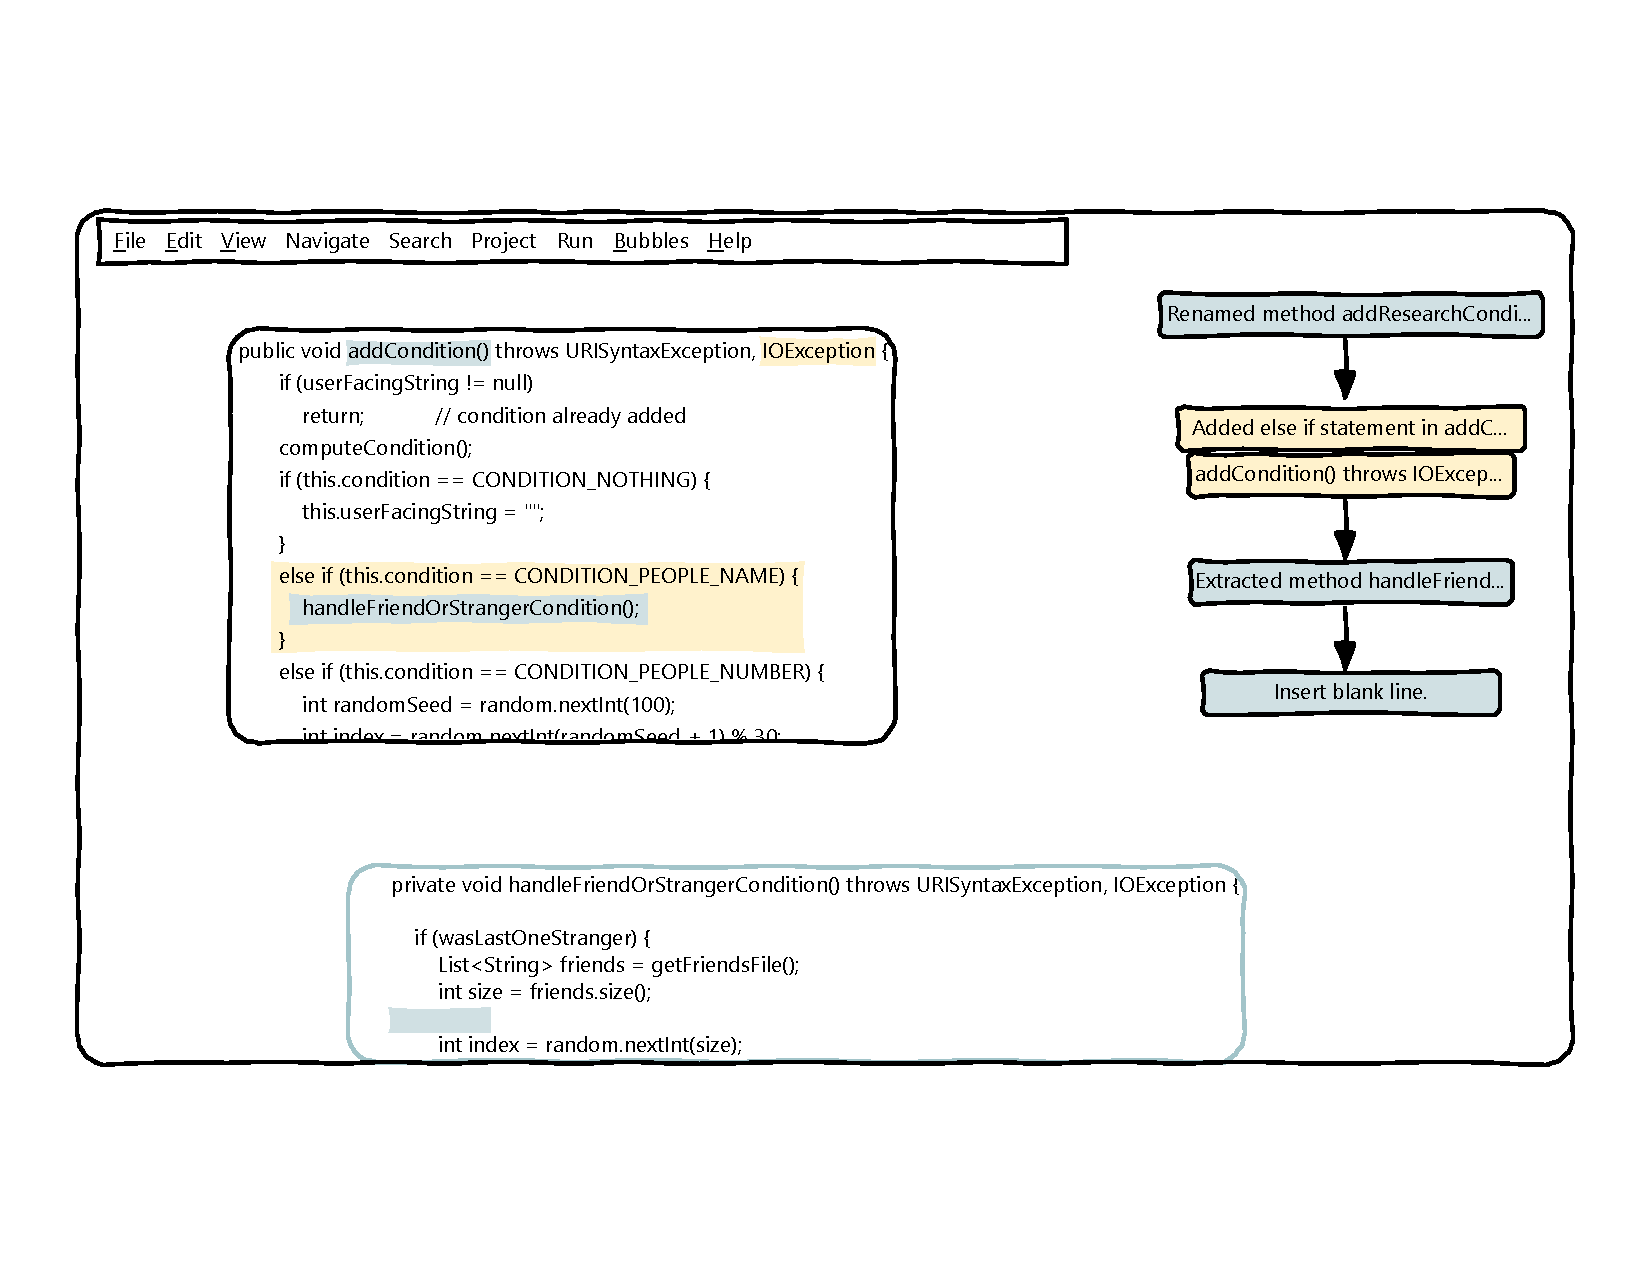
\includegraphics[width=3.5in]{commit-bubbles}
\caption{A mockup of TACO, showing the commit bubbles (A), the mouseovers (B),
and the change notifications (C)}
\label{fig:eclipse}
\end{figure}
\subsection{Commit Bubbles}
As a developer writes code, the IDE detects changes to the AST and autogenerates small commits
that conform to the one commit = one change rule.
These autocommits are placed in bubbles ordered chronologically from the top down.
The colors of the bubble indicate the type of commit; in this example, green commits mean nothing
semantic happened (e.g. refactoring) and yellow commits indicate logic changes.
These autogenerated messages are meant to help the developer remember roughly what happened and
easily deal with trivial commits and they are free to change the messages to suit their needs.

At any time, the developer may drag these commit bubbles around to reorder the history of the code,
combine two or more bubbles into one bigger feature set, do a \textit{soft delete}
or a \textit{hard delete} of one of the bubbles.
If a developer soft deletes a commit bubble, it won't go into the published history, but will still be a temporary artifact of their code base.
Suppose Jim, our example developer from earlier, wishes to insert some log statements or perform
some other test changes while debugging.  
Soft deleting allows him to prune the public history of these debugging artifacts, while still maintaining them in his code.
Hard deletions remove both the commit bubble and the corresponding code segments from the code base and the history. 

Developers clear these commit bubbles out when they press the ``commit'' button, saving them in the VCS.  
For a short while afterwards, they may undo this commit, repopulating the commit bubbles, allowing them to change their minds about what was saved to the public history.
\subsection{Synchronized mouseovers}
As each commit bubble is made, a small colored overlay appears next to the lines with the corresponding change.
These overlays offer developers a visual cue as to how much code has been changed since they 
committed their last set of commit bubbles.
Mousing over these overlays highlights the appropriate code bubble or bubbles,
reminding developers what changes occurred.

There is a temporal aspect of these overlays as well.
If more than one commit bubble impacts a line of code, the overlays stack
themselves left to right, helping keep the recent history in the mind of 
the developer.

\subsection{External Change notifications}
Software developed by groups of people can be prone to the same piece of code
being modified by multiple people at the same time.
TACO watches the public history of the code base and warns developers
of potential conflicts as they type.  
This way, merge conflicts can be dealt with earlier, rather than later.
Additionally, if the development team is collaborating using TACO, they
may also be notified if refactorings like file renames may impact their work, again, allowing earlier responses and easier resolutions.

\section{Example User Experience}
Software Developer Anthony is investigating a bug report about the Eclipse JDT crashing with a NullPointerException
He follows the stack trace to a method shouldIgnoreOptionalProblems, a method he hasn't worked with before.
The stacktrace doesn't indicate which variable was null, so Anthony decides to improve readability and debugability 
to the code by extracting the broken logic to a self-explaining method isParentOf.
Anthony adds in a few debug print statements (resulting in the code in Figure \ref{fig:eclipse}) and then writes a test replicating 
the steps in the bug report.
The print statements indicate that a null fileName is the root cause, so Anthony adds in an additional check,
leaving his commit bubbles looking like Figure \ref{fig:bubblesAfterCheck}.
%TODO insert bubblesAfterCheck here
%The history looks something like: extract method isParentOf; moved for loop to isParentOf;
% adds debug statements;writes a test; adds null check

At this point his history is a bit of a mess, so Anthony decides to reorganize it.
First, he drags the creation of the unit test to the beginning where it is supposed to go, as per TDD standards.
%TODO insert reorder figure
%The history looks something like: writes a test; extract method isParentOf; moved for loop to isParentOf;
% adds debug statements; adds null check
Anthony doesn't want his debug statements in production, but he might still need them,
 so he breaks those out into his private branch with a simple drag gesture.
%TODO insert breakout figure
%The history looks something like: writes a test; extract method isParentOf; moved for loop to isParentOf;
% adds null check   | adds debug statements; 
Finally, he combines the two refactoring bubbles into one because they were both needed to properly extract
the logic of isParentOf.
%TODO insert merge figure
%The history looks something like: writes a test; (extract method isParentOf; moved for loop to isParentOf;)
% adds null check   | adds debug statements; 
He adjusts the name of the merged bubble, leaving his history as in Figure \ref{fig:fixedHistory} presses commit.
%TODO final figure
%The history looks something like: writes a test; (extract method isParentOf; moved for loop to isParentOf;) renamed to Extracted directory comparison to isParentOf
% adds null check   | adds debug statements; 

\section{Concrete Approach in Eclipse / Future Work}

eclipse plugin using http://www.eclipse.org/jgit/
ecj <-- ast
hooking into tools extension point to capture tool commands

%\section{Introduction}

%TODO are all of these things change tasks

%computers -- designed for productivity?

%ideas are ``integrated'', yet their tools are compartmentalized.

%version control systems.
%they are difficult because of compartmentalization vs. integration? (what is the cognitive theory for this?)

%examples of how they are different:

%evolution of flow in tools -> compartment to integrated

%proposed model -> integration as first class principle

%semantic resolution of the tool is different from the semantic resolution of the system

%screen capture of a mockup demonstrating this concept

\section{Related Work}

Bento box design~\cite{DeLine2010a}

refactoring edit history of source code~\cite{Hayashi2012}

why is this citation here? ``Messages written by programmers in version-control commit logs do not reliably indicate the presence of refactoring in the commit.''
floss versus root canal refactoring~\cite{Murphy-Hill2012c}

intro -- need more papers on comprehension during change maintenance tasks

techniques we can leverage?
inserts vertical whitespaces into code to improve readability~\cite{Wang2011}


talk about \emph{task context} model

stylecop
and today! https://gitcop.com/

% TODO make a workflow figure

maybe in introduction -- influence on tasks on programming behavior~\cite{Ying2011a}

also in introduction -- automatic segmentation of method code into
meaningful blocks to improve readability 

what's wrong with git. what are some problems and how do we know?~\cite{PerezDeRosso2013}

Wingerd and Seiwald
high-level best practices in software configuration management~\cite{Wingerd1998}

Coven combines features in a collaborative setting; probably closes in spirit to the type of thing that we're trying to accomplish.~\cite{Chu-Carroll2000}

crosscutting system artifacts
posits that many development tasks do have structure
launch point because it has a lot of good citations
task alignment?~\cite{Murphy2005}

some ncie fragments; mockup; structure on multidimensionality; again lock focused (hierarchical locking -- not a model needed anymore)
~\cite{Chu-Carroll2003}

infuse, ``experimental databases'', managing and coordinating source code changes; introduces term \emph{change propagation}~\cite{Perry1987}

inscape environment = ``Dividing the life-cycle into two distinct phases, development and maintenance, introduces a distinction that is not born out in practice.'' and ``tools that are knowledgeable about the process of system construction and evolution and work in symbiosis with the system builders and evolvers'' paper focuses a lot on formal specifications.~\cite{Perry1989}


% http://delivery.acm.org.prox.lib.ncsu.edu/10.1145/360000/355058/p88-chu-carroll.pdf?ip=152.14.136.96&id=355058&acc=ACTIVE%20SERVICE&key=6ABC8B4C00F6EE47.4D4702B0C3E38B35.4D4702B0C3E38B35.4D4702B0C3E38B35&CFID=596113106&CFTOKEN=10420211&__acm__=1415544717_ebea3078944a1cffe21be1875ddc99c8

% http://dl.acm.org.prox.lib.ncsu.edu/citation.cfm?id=1321647

% http://dl.acm.org.prox.lib.ncsu.edu/citation.cfm?id=605482

% http://ieeexplore.ieee.org.prox.lib.ncsu.edu/xpls/abs_all.jsp?arnumber=4509441&tag=1

TODO: model-driven engineering, is that the same? START HERE
 --> right model for person, not for computer
% http://www.emeraldinsight.com.prox.lib.ncsu.edu/doi/abs/10.1108/17440080910983556

% http://e-collection.library.ethz.ch/eserv.php?pid=eth:46754&dsID=eth-46754-01.pdf


\section{State of the world today}

auto-complete, flow breaking activity when writing commit messages because of lack of semantic information

run builds not on your repository but against last commit + change

light stacking system for changes

\section{Our approach}

git as a version control framework, not a version control system

- what are some other models of this
- legit? git-flow? superimpose model on API
http://www.eclipse.org/jgit/ <-- nice option for how to implement this

\footnote{\url{http://www.eclipse.org/jgit/}}

\section{Challenges}

-- implementation?
naive should be easy: capture tool usage directly  
hard: ghostfactor (changes without using tools) , but other people
 are addressing this: See 1, 2, 3 for better semantic support which our tools will be able to leverage
 
 - worst-case combinatorial, but look at techniques more pruning this space using common design patterns, heuristics (temporal heuristics) (accuracy of temporaral heuristics)
 
 -- minimal screen resolution, passive information, always-on vs. on-demand? CPU performance. ui management across multiple files. higher level operations --> rename, delete files.
 -- changes not in the IDE
 -- does everyone have to use the tool? what if they don't? do we lose all support?

 -- what if you need the low-level? you no longer have any mental model between the two
 
 http://importantshock.wordpress.com/2008/08/07/git-vs-mercurial/


\section{Conclusion}


need a nice concept for framing

\begin{figure}[!t]
\centering
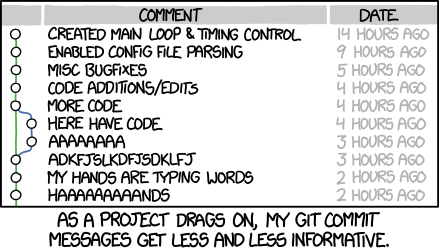
\includegraphics[width=\linewidth]{xkcd}
\caption{This is part of the problem.}
\label{fig:xkcd}
\end{figure}

% An example of a floating table. Note that, for IEEE style tables, the
% \caption command should come BEFORE the table. Table text will default to
% \footnotesize as IEEE normally uses this smaller font for tables.
% The \label must come after \caption as always.
%
%\begin{table}[!t]
%% increase table row spacing, adjust to taste
%\renewcommand{\arraystretch}{1.3}
% if using array.sty, it might be a good idea to tweak the value of
% \extrarowheight as needed to properly center the text within the cells
%\caption{An Example of a Table}
%\label{table_example}
%\centering
%% Some packages, such as MDW tools, offer better commands for making tables
%% than the plain LaTeX2e tabular which is used here.
%\begin{tabular}{|c||c|}
%\hline
%One & Two\\
%\hline
%Three & Four\\
%\hline
%\end{tabular}
%\end{table}


% Note that IEEE does not put floats in the very first column - or typically
% anywhere on the first page for that matter. Also, in-text middle ("here")
% positioning is not used. Most IEEE journals/conferences use top floats
% exclusively. Note that, LaTeX2e, unlike IEEE journals/conferences, places
% footnotes above bottom floats. This can be corrected via the \fnbelowfloat
% command of the stfloats package.

% use section* for acknowledgement
\section*{Acknowledgments}

I did this all by myself.


% trigger a \newpage just before the given reference
% number - used to balance the columns on the last page
% adjust value as needed - may need to be readjusted if
% the document is modified later
%\IEEEtriggeratref{8}
% The "triggered" command can be changed if desired:
%\IEEEtriggercmd{\enlargethispage{-5in}}

% references section

% can use a bibliography generated by BibTeX as a .bbl file
% BibTeX documentation can be easily obtained at:
% http://www.ctan.org/tex-archive/biblio/bibtex/contrib/doc/
% The IEEEtran BibTeX style support page is at:
% http://www.michaelshell.org/tex/ieeetran/bibtex/
\bibliographystyle{IEEEtran}
% argument is your BibTeX string definitions and bibliography database(s)
\bibliography{library}



% that's all folks
\end{document}


